\section{\ttt{3D} Classification and Refinement}

 \begin{figure}[H]
  \centering
  \captionsetup{width=.8\linewidth} 
  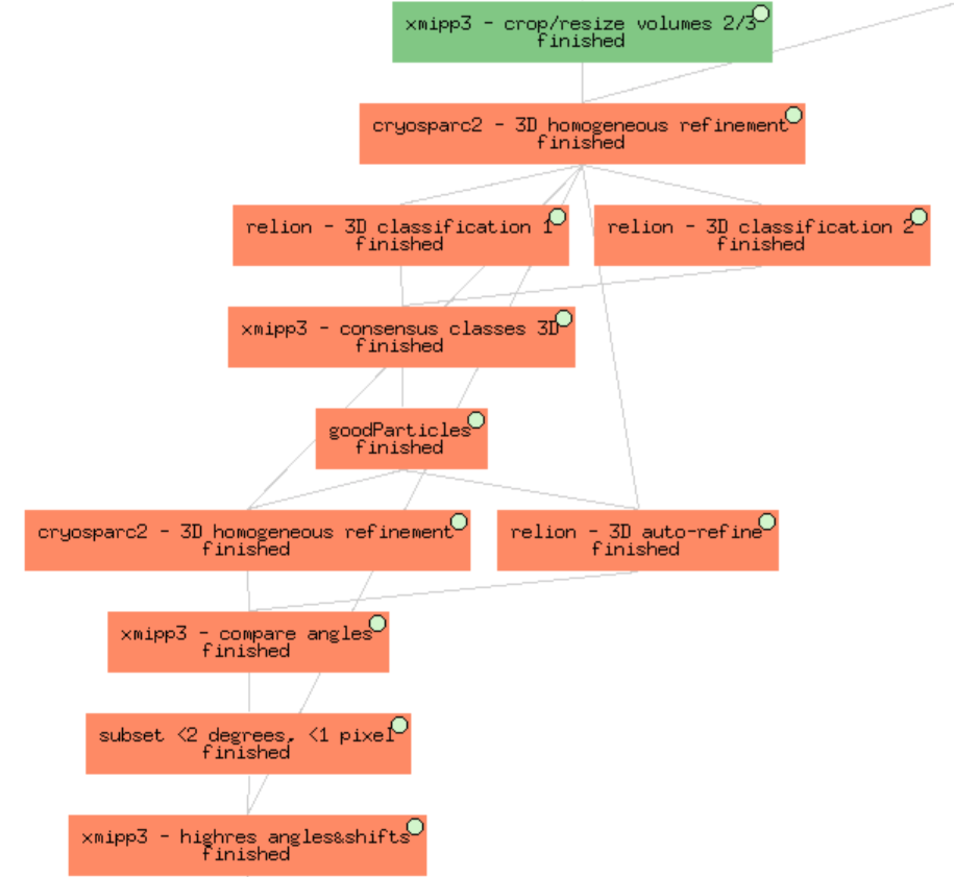
\includegraphics[width=1\textwidth]
  {{images/9_workflow7_3D_RandC.pdf}}
  \caption{Refinement and \ttt{3D} Classification.}
  \label{fig:workflow_7}
  \end{figure}

\ttt{3D} Classification and Refinement are the two last overlapping steps in image processing. They consume the most time and resources with the aim of obtaining a \ttt{3D} map at the highest possible resolution. This is only feasible if data is homogeneous enough, $i.e.$, if data represent a unique conformation of the specimen.\\

\subsection*{Refinement of the initial map}
Before starting with the \ttt{3D} classification properly, a refinement step will be performed with our initial map. The first approach to get a high resolution map in a fully automated manner was performed with the algorithm $Cryosparc$ \ttt{homogenous refinement}. This procedure rapidly refines a single homogeneous structure to high-resolution and validate using the gold-standard Fourier Shell Correlation (FSC). We have implemented it in the protocol \scommand{cryosparc2-homogeneous refinement} (\ffigure{fig:cryosparc_refine}). In the \ttt{Input} tap of this protocol form we include the subset of homogeneous particles extracted previously and the initial volume computed, as well in the \ttt{Refinement} tap we will choose the symmetry (octahedral), we will select all the options and we will choose in \ttt{Noise model} symmetric. 

\begin{figure}[H]
  \centering
  \captionsetup{width=.8\linewidth} 
  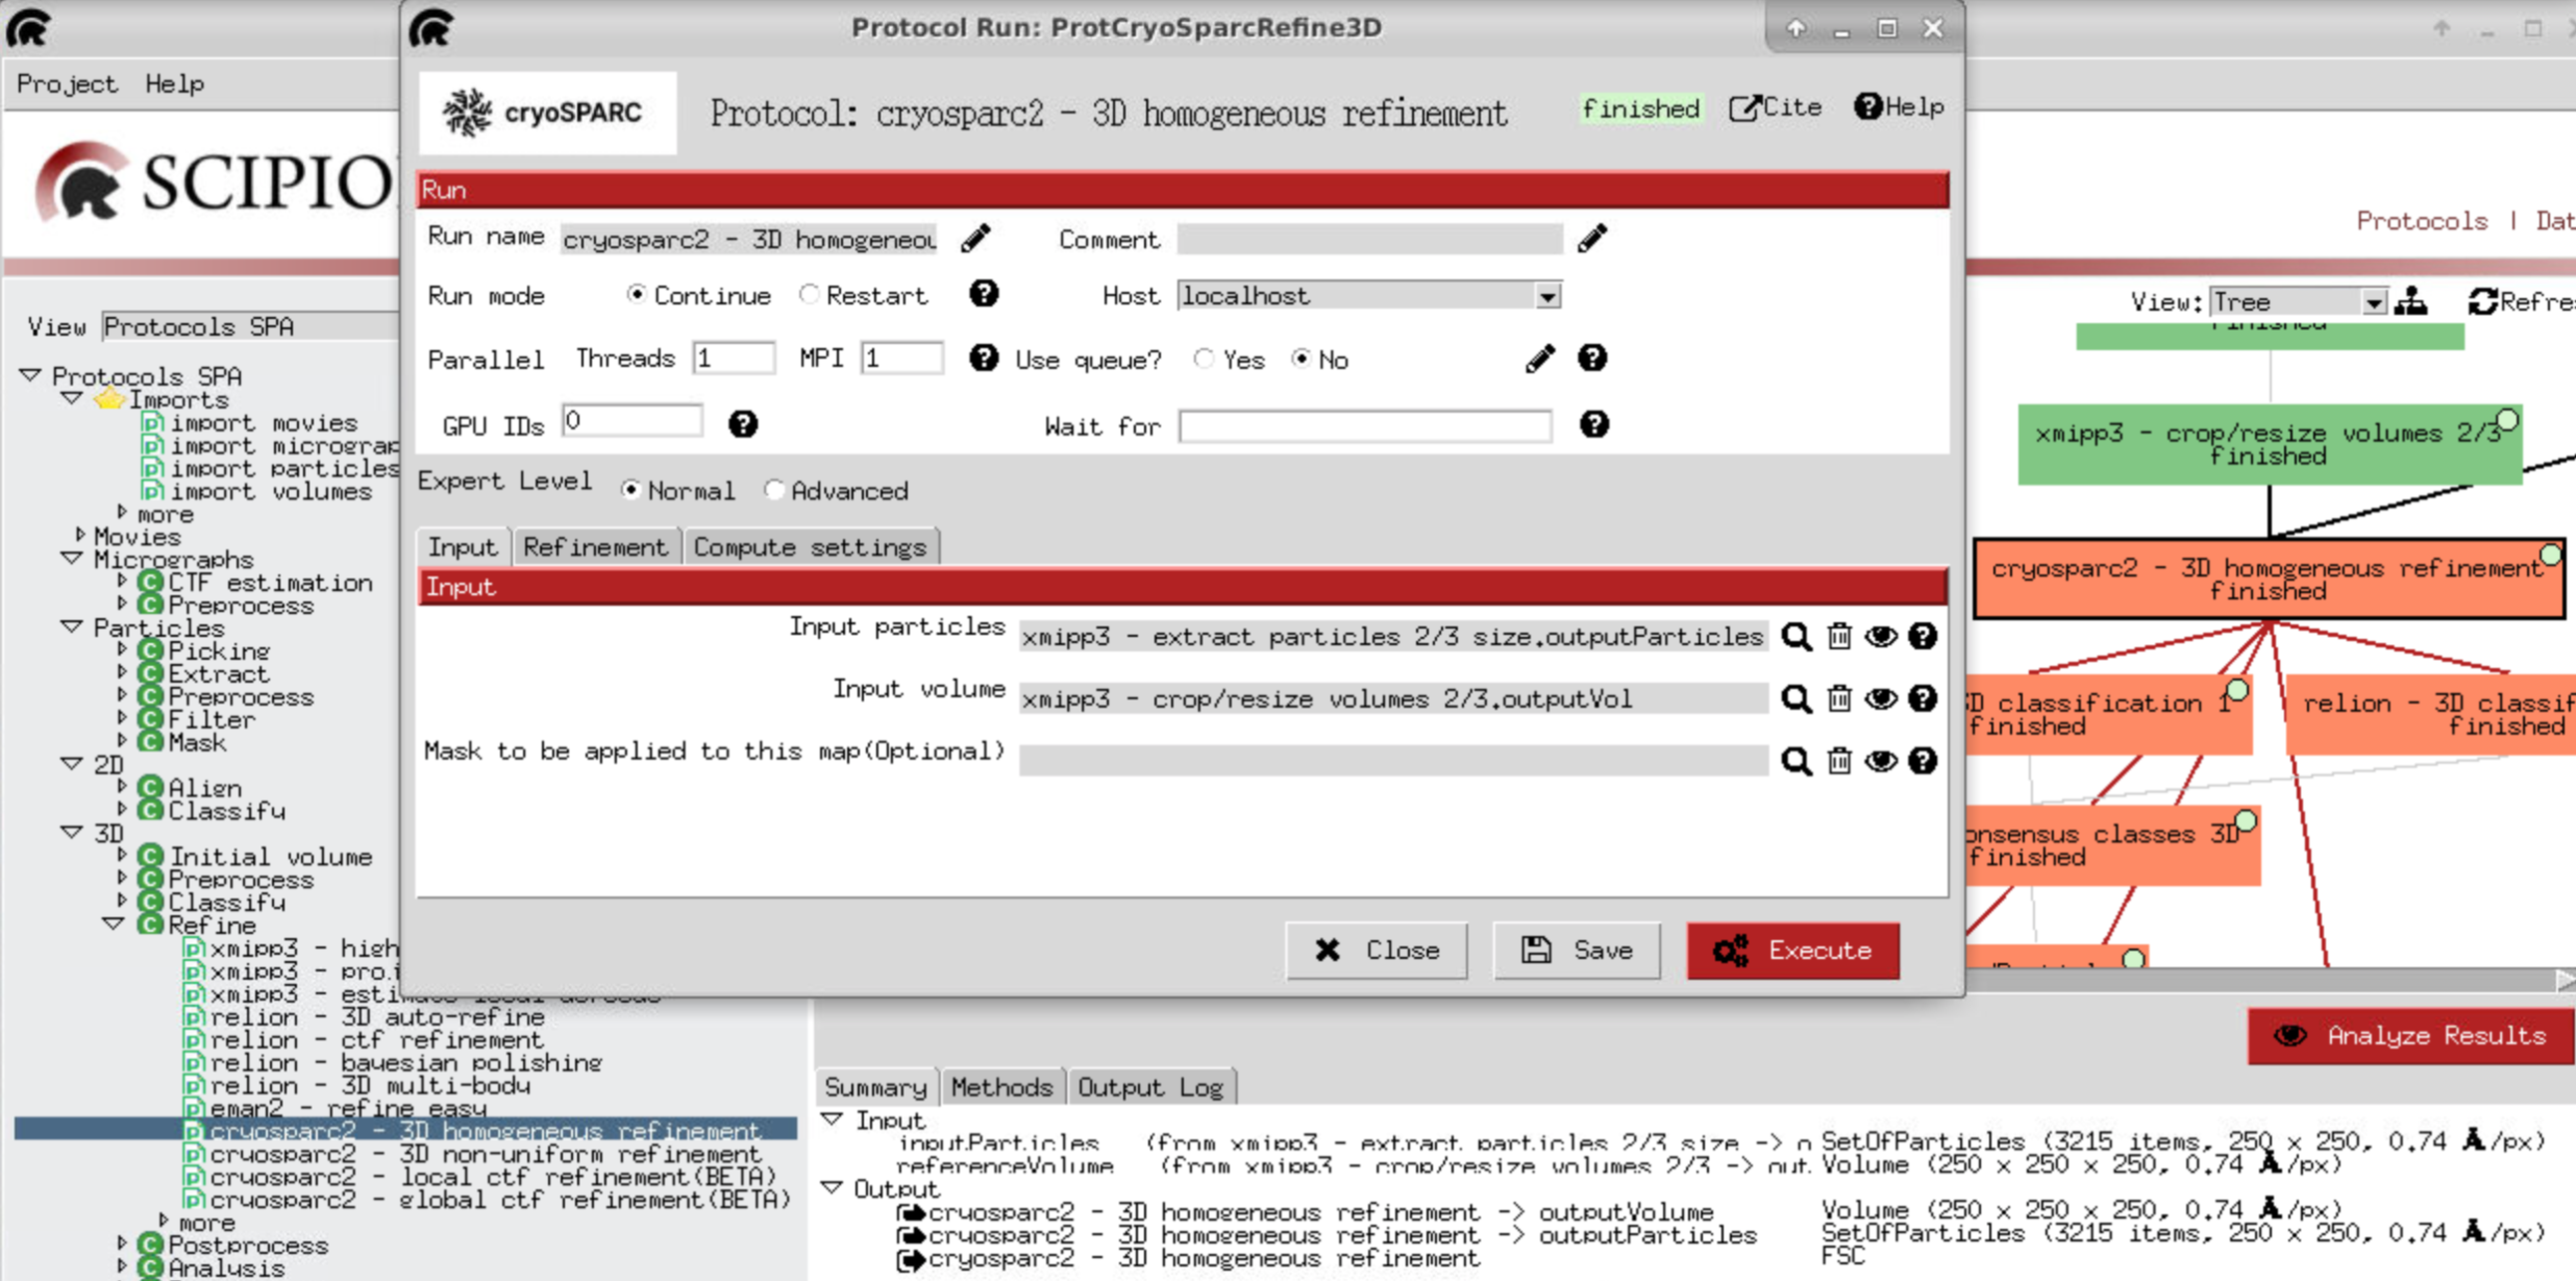
\includegraphics[width=0.95\textwidth]
  {{images/9a_cryosparc2_3Dhrefinement.pdf}}
  \caption{Completing the params of the protocol \scommand{cryosparc2-homogeneous refinement}.}
  \label{fig:cryosparc_refine}
  \end{figure}

After executing, a refined map of 3.3 \AA\ of final resolution was obtained as output, with the same size and sampling rate that we had in the inputs. Press \scommand{Analyze Results} to visualize the FSC, the volume or the set of particles. With our initial volume and set of particles we can see that it nicely converge in a good 3D structure, however, we do not know if all the particles that we have used are consistent with that structure and we also do not know if the parameters of those have been correctly identified. These would be tried to be solved in the next section.

\subsection*{3D classification}
To continue with the refinement process to obtain a better resolution and to answer the first question, if all the particles belong to that structure, we start executing two independent times the same algorithm of $Relion$ \ttt{3D classification} that we have implemented in the protocol \scommand{relion-3D classification} (\ffigure{fig:relion_3Dclassification}). In the tap \ttt{Input} we include the particles derived from executing the previous protocol \scommand{cryosparc2-homogeneous refinement}. The volume derived from this protocol will be the \ttt{Input volume(s)} in the tap \ttt{Reference 3D map} and will be low-pass filtered by 15\AA\ . The optimization params appear in the tap \ttt{Optimization}: 2 \ttt{Number of classes} and 25 \ttt{Number of iterations}. As \ttt{Regularisation parameter T} values as 3-4 are common for \ttt{3D} classification.

\begin{figure}[H]
  \centering
  \captionsetup{width=.8\linewidth} 
  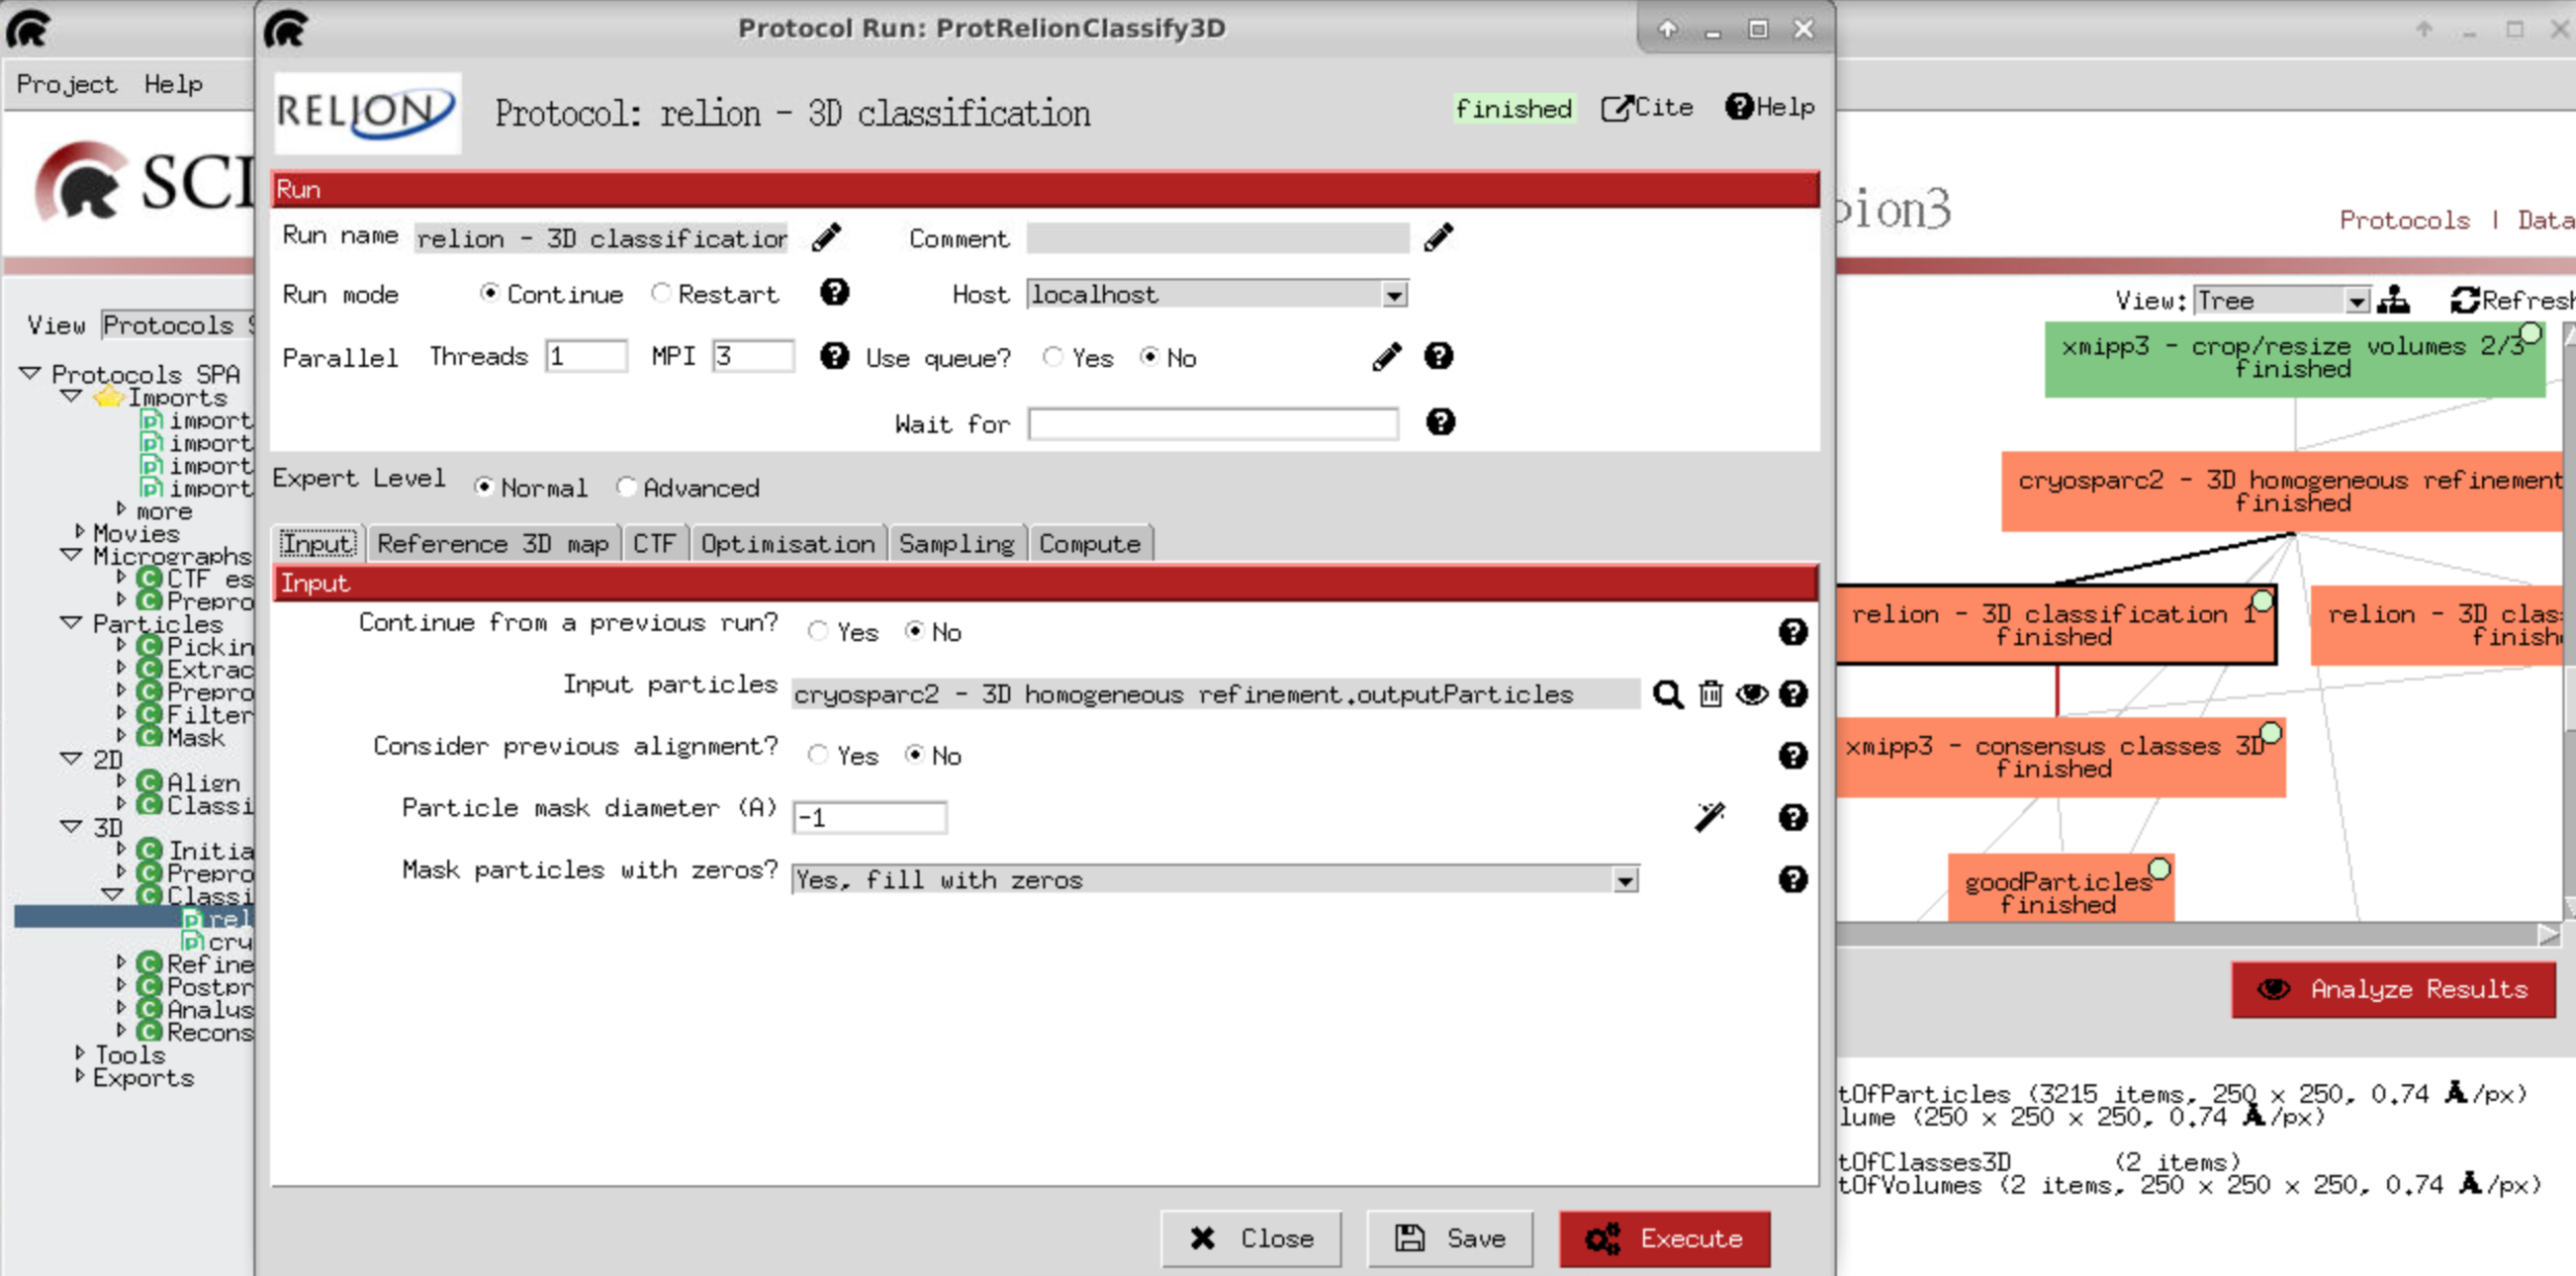
\includegraphics[width=0.95\textwidth]
  {{images/9b_relion_3DClassf_1.pdf}}
  \caption{Completing the params of the protocol \scommand{relion-3D classification}.}
  \label{fig:relion_3Dclassification}
  \end{figure}
  
The output of each one of these two \scommand{relion-3D classification} protocols are 2 maps with the initial size and sampling rate, reconstructed from different groups of reclassified particles. By pressing \scommand{Analyze Results} and \ttt{Particles/ Show classification in Scipion}, a table will be opened showing the projection representative of each map and the number of particles contributing to its reconstruction:
\begin{itemize}
 \item 2,428 and 787 in the first classification.
 \item 2,460 and 755 in the second one.
\end{itemize}

The results of the first and second \ttt{3D} classifications are similar, in both cases the first class contains most of the particles. In order to have a consensus of these results, we execute the protocol \scommand{xmipp3-consensus classes 3D} that compares several sets of \ttt{3D} classes and return the intersection of the input classes (\ffigure{fig:consensus_classes}).

\begin{figure}[H]
  \centering
  \captionsetup{width=.8\linewidth} 
  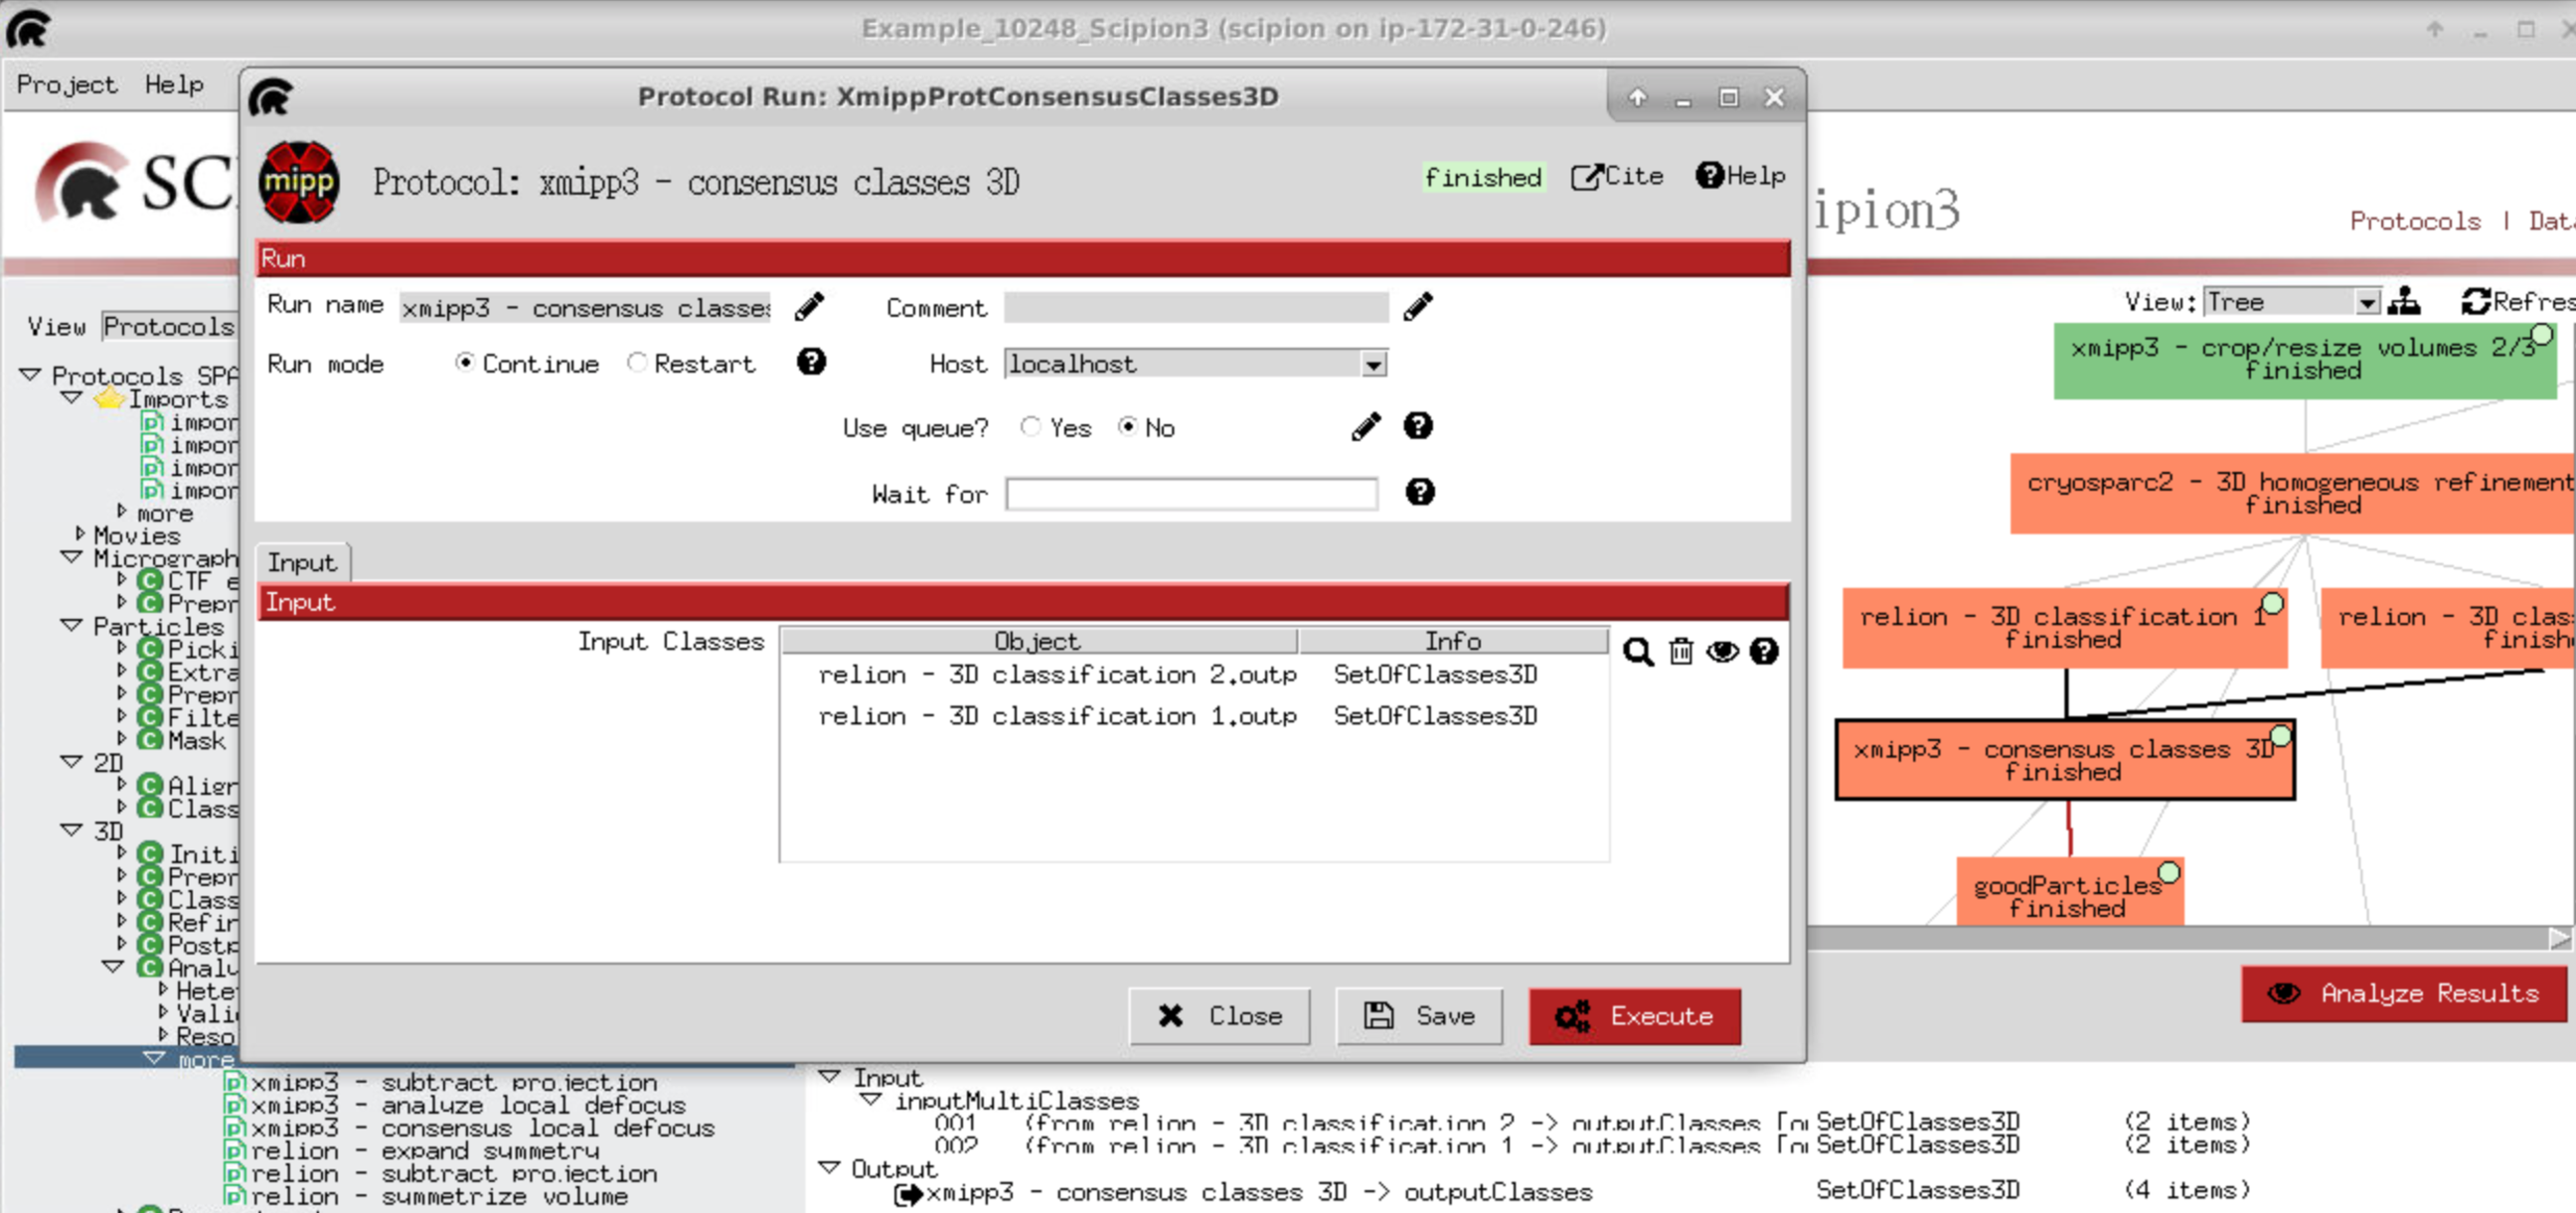
\includegraphics[width=0.95\textwidth]
  {{images/9d_xmipp3_3Dconsensus.pdf}}
  \caption{Filling in the params of the protocol \scommand{xmipp3-consensus classes 3D}.}
  \label{fig:consensus_classes}
  \end{figure}
  
By pressing \scommand{Analysis Results} you can visualize the 4 intersection \ttt{3D} classes with the number of particles assigned to each one. The first of these classes derive from about 1,944 particles (aprox. 60\% of total particles). Once inspected the different classes, by selecting the classes that we are interested in (only the first one) and pressing \scommand{Particles}, a new subset of 1,944 particles will be created included in the box \ttt{goodParticles}.

\subsection*{Refinement}

For a further refinement step, we will use again the protocol \scommand{cryosparc2-homogeneous refinement} (\ffigure{fig:cryosparc_refine2}) and $Relion$ algorithm \ttt{3D auto-refine} that we have implemented in the protocol \scommand{relion-3D auto-refine} (\ffigure{fig:relion_3Dautorefine}). As input, we include the set of good particles that were consistently assigned to the same class and the initial volume computed in the step before.   

\begin{figure}[H]
  \centering
  \captionsetup{width=.8\linewidth} 
  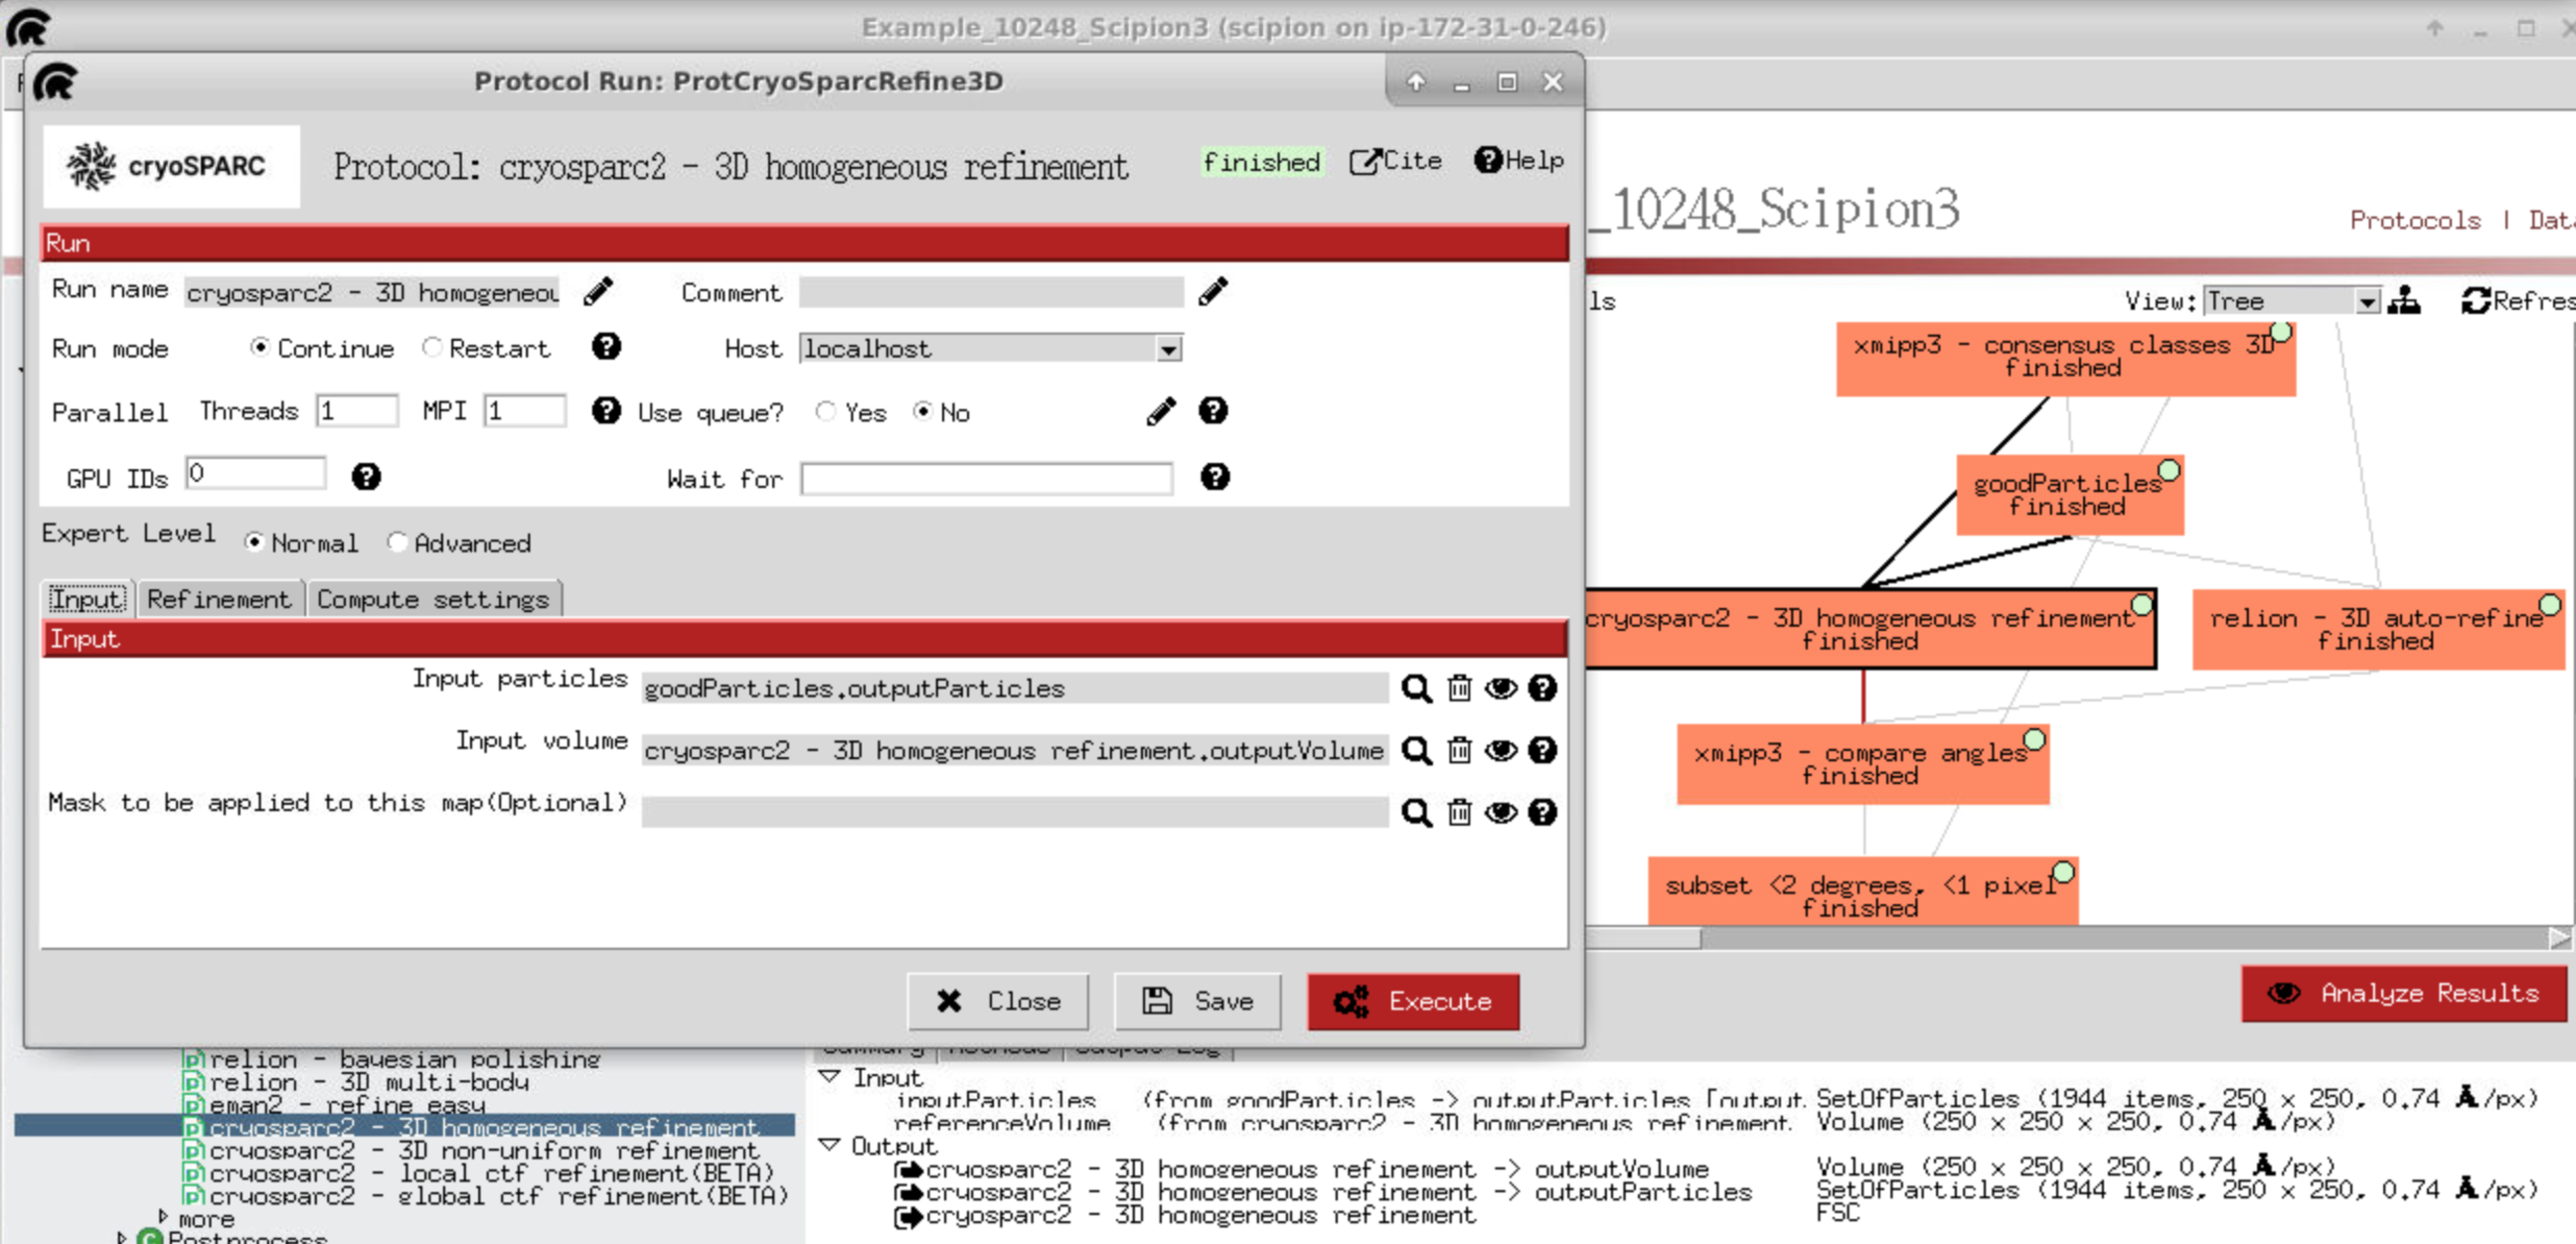
\includegraphics[width=0.95\textwidth]
  {{images/9e_cryosparc2_3Drefinement2.pdf}}
  \caption{Completing params of protocol \scommand{cryosparc2-homogeneous refinement}.}
  \label{fig:cryosparc_refine2}
  \end{figure}
  
 The algorithm of $Relion$ \ttt{auto\_refine}, is based on an empirical Bayesian approach. This procedure employs the so-called gold-standard Fourier Shell Correlation (FSC) to estimate the resolution. Combined with a novel procedure to estimate the accuracy of the angular assignments, the algorithm converges. In the \ttt{Input} tap of this protocol form we include the subset of good particles selected previously. The initial volume in the \ttt{Reference 3D map} tap and as we trust our previous map we do not need to filter it much so we apply a \ttt{Initial low pass-filter (A)} of 10.0 \AA\ .  This tap gives you the possibility of using \ttt{Reference mask (optional)}.
 
 \begin{figure}[H]
  \centering
  \captionsetup{width=.8\linewidth} 
  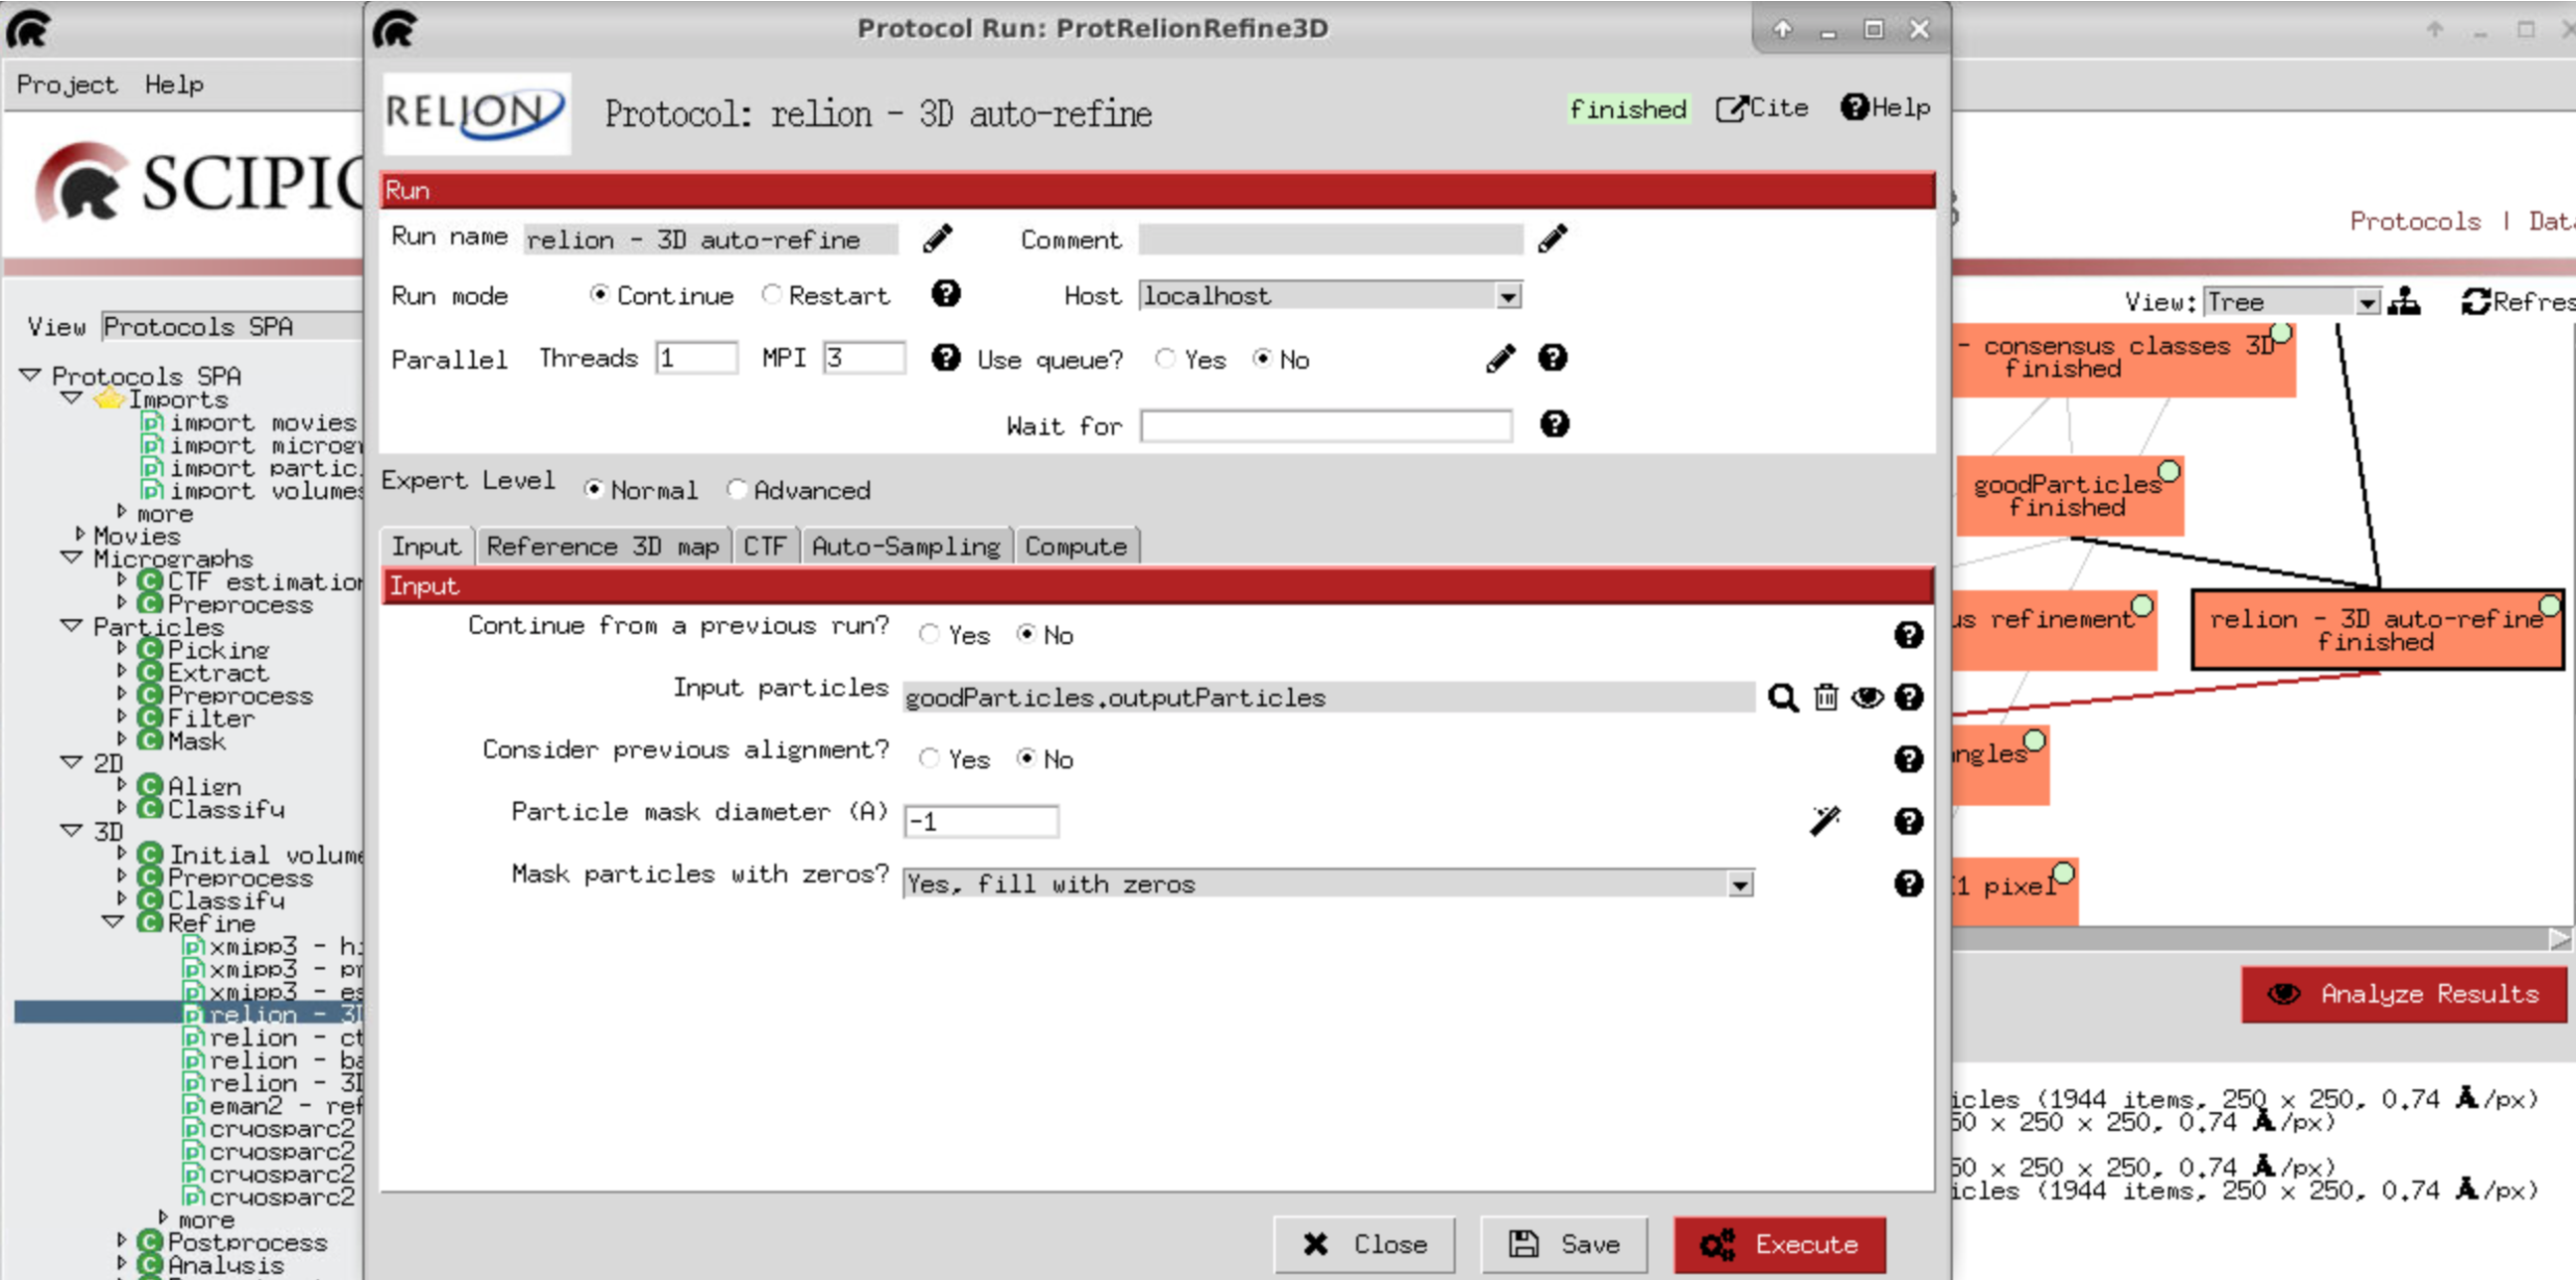
\includegraphics[width=0.95\textwidth]
  {{images/9f_relion_3Dautorefine.pdf}}
  \caption{Completing params of protocol \scommand{relion-3D auto-refine} .}
  \label{fig:relion_3Dautorefine}
  \end{figure} 
  
There are three questions in the tab \ttt{CTF}: 
\begin{itemize}
 \item \ttt{Do CTF correction?}, set to \ttt{Yes} to perform full phase + amplitude CTF correction.
 \item \ttt{Has reference been CTF-corrected?}, set to \ttt{No} because the Fourier transforms of the reference projections are not multiplied by the \ttt{CTF} in the first iteration. 
 \item \ttt{Do manual grouping ctfs?}, set to \ttt{No} because we have enough number of particles that we do not need to group them.
\end{itemize}

The \ttt{Angular sampling interval (deg)} option in the tab \ttt{Auto-Sampling} will be used only in the first few iterations. Later, the algorithm will automatically increase its value until convergence. For symmetries lower than octahedral or icosahedral we use the default values of \ttt{Angular sampling interval (deg)} and \ttt{Local search from auto-sampling (deg)}.\\

After executing both protocols, by looking to the resolution \ttt{FSC} plots, a refined map of 2.8-3\AA\ of final resolution was obtained as output, with the same size and sampling rate that we had in the inputs. Press \scommand{Analyze Results} and by comparing the output volumes same slices, we can visually see the difference between the two maps obtained by the two protocols. In this particular case, we observe haze on top of relion output volume and this typically is coming from badly align particles. To identify these badly align particles, we can compare the angular assignment of relion and cryosparc protocols using \scommand{xmipp3-compare angles} protocol  (\ffigure{fig:xmipp_compareAngles}). As we have an octahedral symmetry we do not have to align the volumes. If needed, you can use \scommand{xmipp3-align volume and particles} protocol.

 \begin{figure}[H]
  \centering
  \captionsetup{width=.8\linewidth} 
  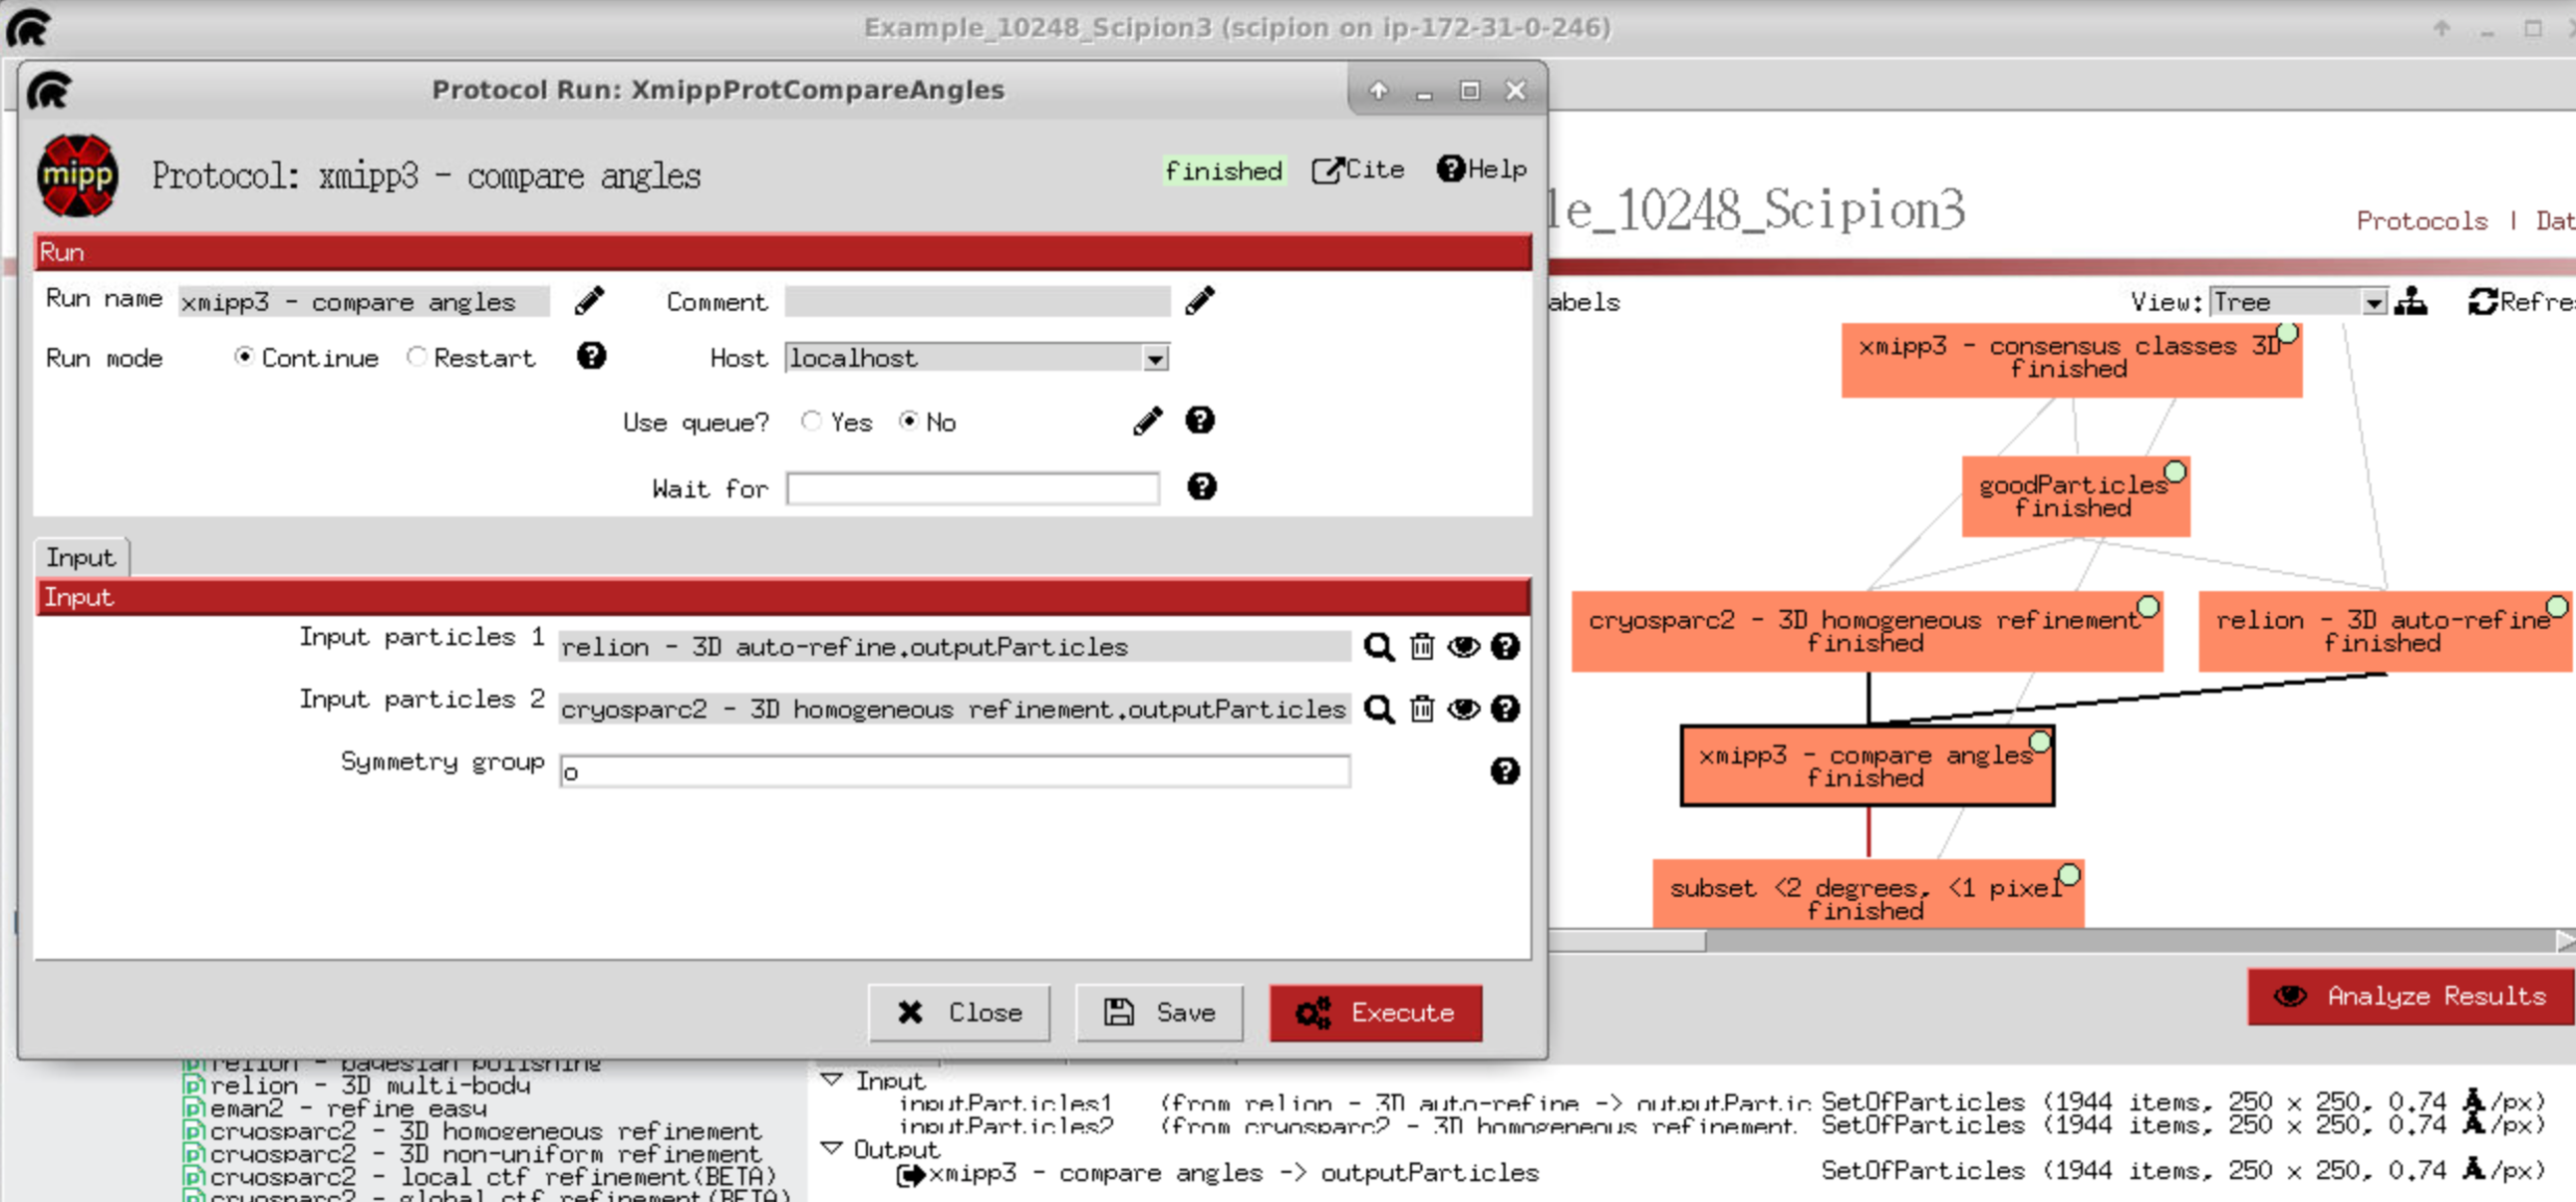
\includegraphics[width=0.95\textwidth]
  {{images/9g_xmipp3_compareangles.pdf}}
  \caption{Completing params of protocol \scommand{xmipp3-compare angles} .}
  \label{fig:xmipp_compareAngles}
  \end{figure} 
  
  The results given is a set of particles sorted by the angular difference, and for every particle we have its angular difference (average of the Euler angles) and the shift difference. As they are sorted, if we plot the column of angular difference we can observe that most are around 1 degree difference. However, there are others that the angular error is much bigger and those are the particles that their angular assignment is not so convincing. If we select the ones below 2 degree differences, sort by angular shift, repeat the process and select those below 1 pixel shift, we will create a new subset (1,903) whose particles have an angular assignment consistent between two algorithms (relion and cryosparc) with different implementations. Then, we proceed to make the angular reassignment of this new subset of particles to our refined map of protocol \scommand{cryosparc2-homogeneous refinement} (\ffigure{fig:cryosparc_refine}) using the $Xmipp$ algorithm \ttt{highres} \citep{sorzano2018new} that we have implemented in the protocol \scommand{xmipp3-highres} (\ffigure{fig:xmipp_highres_1}).\\ 
  
 This method computes a weight for each particle and performs both global or local alignment. Iterations can be performed one by one, removing particles that worse fit the map from one iteration to the next one. This \ttt{3D} refinement protocol uses as input the refined map obtained from $Cryosparc$ \ttt{homogenous refinement} and the subset of particles created before. The \ttt{Symmetry group} has been also included in the \ttt{Input} tap. In the \ttt{Angular assignment} tap we choose \ttt{Local} as \ttt{Image alignment} as we have a previous estimated assignment computed before, and 1 \ttt{Number of iterations} with 2 \AA\ as \ttt{Max. Target Resolution}. In this particular case, as we have few data it is not recommended to optimize the scale, the grey values or the defocus. 
 
  \begin{figure}[H]
  \centering
  \captionsetup{width=.8\linewidth} 
  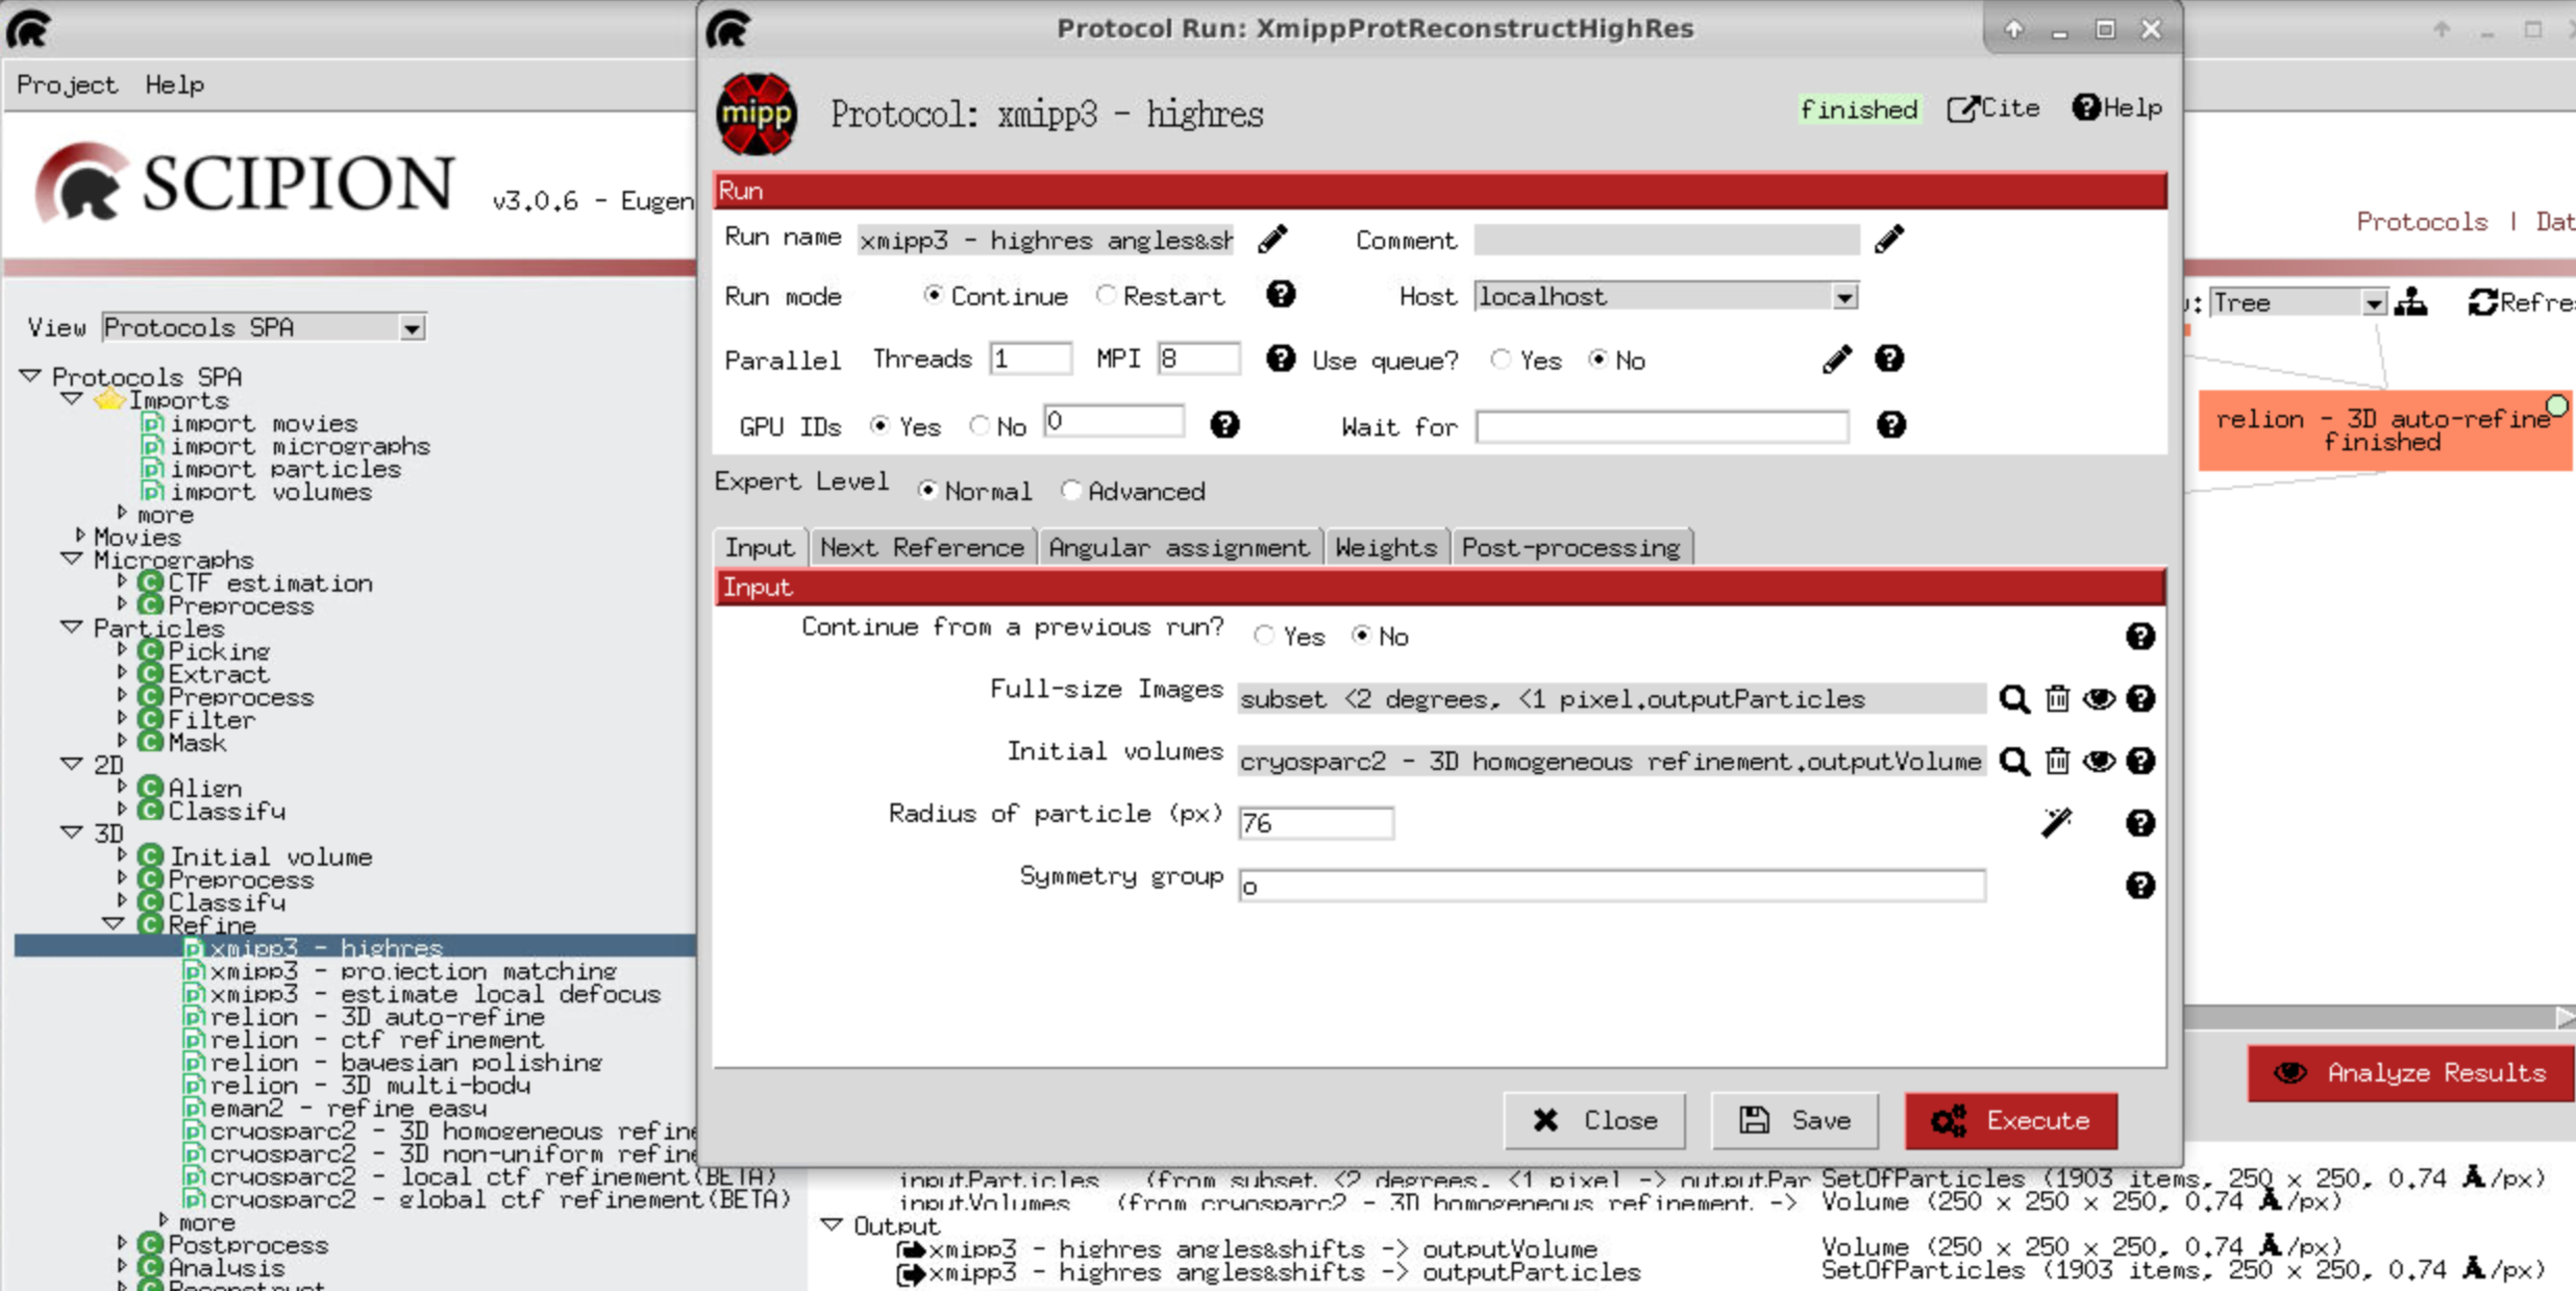
\includegraphics[width=0.95\textwidth]
  {{images/9h_xmipp3_highres.pdf}}
  \caption{$Xmipp$ \ttt{highres} map local refinement.}
  \label{fig:xmipp_highres_1}
  \end{figure}
 
This protocol generates one map as output with the initial size and sampling rate. Press \scommand{Analyze Results} to check the results. Particles and map can be visualized. We can observe that no particles have been rejected. The output resolution by displaying the FSC, is around 3.2\AA . We can select particles according to the value of the \ttt{\_xmipp\_cost} param and we can observe the angular distribution. The output volume obtained looks very good, we get rid off the haze and if we can appreciate more details in the 3D structure. In the next section, we will see how to validate our processing and to enhance the volume obtained with this workflow.\\

  For more information: 
\begin{itemize}
   \item \textbf{Video tutorial}:  \url{https://www.youtube.com/watch?v=ial95OZJXU0&list=PLQjWIcrmtc4JjyC-_BM99_XW-VsDa4_i3&index=29}.
   \item \textbf{Theoretical lecture}:  \url{https://www.youtube.com/watch?v=taCREkFAPoE&list=PLQjWIcrmtc4JjyC-_BM99_XW-VsDa4_i3&index=36}.
  \end{itemize}           

